\renewcommand{\thetheorem}{25.a.\arabic{theorem}}
\setcounter{theorem}{0}
\setcounter{chapter}{24}

\chapter{Orthogonal and Unitary Maps / Isometries}

\section{Linear Isometries}

% Def. (25.a.1)
\begin{definition}[Linear Isometry]
\label{def:linear_isometry}
Let $V, W$ be inner product spaces over $K$ (where $K = \mathbb{R}$ or $\mathbb{C}$). A map $T \colon V \to W$ is called a \newterm{linear isometry} if $T$ is linear and for all $v_1, v_2 \in V$, 
\[ \langle Tv_1, Tv_2 \rangle_W = \langle v_1, v_2 \rangle_V. \]
(In other words, $T$ preserves the inner product).
\end{definition}

\begin{remark}
If $T \colon V \to W$ is a linear isometry, then:
\begin{enumerate}
    \item For all $v \in V$, $\|Tv\| = \|v\|$.
    \item For all $p, q \in V$, the distance is preserved:
    \[ \dist_W(Tp, Tq) = \|Tp - Tq\|_W = \|p - q\|_V = \dist_V(p, q). \]
    \item $T$ is injective. Indeed, if $v \in \ker T$, then $0 = \|Tv\| = \|v\|$, which implies $v = 0$. So, $\ker T = \{0\}$.
\end{enumerate}

\begin{center}
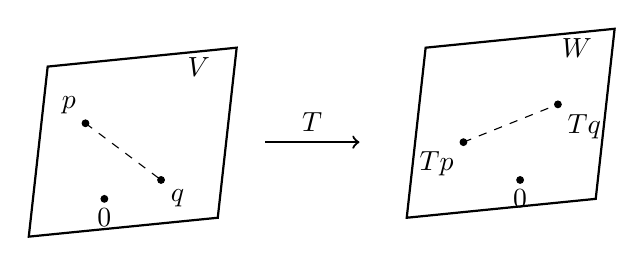
\begin{tikzpicture}[scale=1.2]
    % Space V
    \draw[thick] (0,0) -- (2,0.2) -- (2.2,2) -- (0.2,1.8) -- cycle;
    \node at (1.8, 1.8) {$V$};
    \filldraw (0.6, 1.2) circle (1pt) node[above left] {$p$};
    \filldraw (1.4, 0.6) circle (1pt) node[below right] {$q$};
    \draw[dashed] (0.6, 1.2) -- (1.4, 0.6);
    \filldraw (0.8, 0.4) circle (1pt) node[below] {$0$};

    % Arrow T
    \draw[->, thick] (2.5, 1) -- (3.5, 1) node[midway, above] {$T$};

    % Space W
    \draw[thick] (4,0.2) -- (6,0.4) -- (6.2,2.2) -- (4.2,2) -- cycle;
    \node at (5.8, 2.0) {$W$};
    \filldraw (4.6, 1.0) circle (1pt) node[below left] {$Tp$};
    \filldraw (5.6, 1.4) circle (1pt) node[below right] {$Tq$};
    \draw[dashed] (4.6, 1.0) -- (5.6, 1.4);
    \filldraw (5.2, 0.6) circle (1pt) node[below] {$0$};
\end{tikzpicture}
\end{center}
\end{remark}

From now on, we will concentrate on the case where $W = V$, meaning $T \in \End(V)$. If such a map $T$ is an isometry, we also call it an \newterm{orthogonal endomorphism} if $K = \mathbb{R}$, or a \newterm{unitary endomorphism} if $K = \mathbb{C}$.

% Thm. (25.a.2)
\begin{theorem}[Characterization of Isometries]
\label{thm:isometry_equivalences}
Let $V$ be a finite-di\-men\-sional inner product space over $\mathbb{R}$ or $\mathbb{C}$, and let $T \in \End(V)$. The following statements are equivalent:
\begin{enumerate}
    \item $T$ is an isometry.
    \item For all $v \in V$, $\|Tv\| = \|v\|$.
    \item For every orthonormal system $e_1, \dots, e_k$ of $V$, the list of vectors $Te_1, \dots, Te_k$ is also an orthonormal system.
    \item There exists an orthonormal \emph{basis} $\mathcal{B} := (e_1, \dots, e_n)$ of $V$ such that $Te_1, \dots, Te_n$ is also an orthonormal basis.
    \item $T \circ T^* = \id_V$.
    \item $T^* \circ T = \id_V$.
    \item $T^* = T^{-1}$.
    \item $T^*$ is an isometry.
\end{enumerate}
\end{theorem}

\begin{proof}
We will prove some of the equivalences here; the rest are left as exercises (and for the exercise sheet).

\textbf{(b)} $\implies$ \textbf{(a)}: Using the polarization identity (for the real case), we have:
\begin{align*}
    \langle Tv, Tw \rangle &= \frac{1}{2} \left( \|Tv + Tw\|^2 - \|Tv\|^2 - \|Tw\|^2 \right) \\
    &= \frac{1}{2} \left( \|T(v + w)\|^2 - \|Tv\|^2 - \|Tw\|^2 \right) \\
    &= \frac{1}{2} \left( \|v + w\|^2 - \|v\|^2 - \|w\|^2 \right) \\
    &= \langle v, w \rangle.
\end{align*}

\textbf{(a)} $\implies$ \textbf{(c)}: Let $e_1, \dots, e_k$ be an orthonormal system. Then, for all $1 \leq i, j \leq k$, we have:
\[ \langle Te_i, Te_j \rangle = \langle e_i, e_j \rangle = \delta_{ij}. \]
This implies that $Te_1, \dots, Te_k$ is also an orthonormal system.

\begin{ainote}
In the handwritten notes, the following proof is labeled as \textbf{(d)} $\implies$ \textbf{(e)}. However, it actually proves \textbf{(d)} $\implies$ \textbf{(f)}, which is $T^* \circ T = \id_V$. We have corrected the labeling here.
\end{ainote}

\textbf{(d)} $\implies$ \textbf{(f)}: Let $\mathcal{B} = (e_1, \dots, e_n)$ be an orthonormal basis such that $Te_1, \dots, Te_n$ is also an orthonormal system. Let $1 \leq j \leq n$. We have, for all $1 \leq i \leq n$:
\begin{equation}
    \langle e_i, e_j \rangle = \delta_{ij} = \langle Te_i, Te_j \rangle = \langle e_i, T^*Te_j \rangle. \quad (*)
\end{equation}
Since $(e_1, \dots, e_n)$ is a basis for $V$, the equality $(*)$ implies that by linearity in the first argument,
\[ \langle v, e_j \rangle = \langle v, T^*Te_j \rangle \quad \forall v \in V. \]
This implies that $T^*Te_j = e_j$. This last equality holds for all $1 \leq j \leq n$, which implies that $T^* \circ T = \id_V$.
\end{proof}

\section{Orthogonal and Unitary Matrices}

\noindent
Back to matrices. Recall that:
\begin{itemize}
    \item $A \in \M_{n \times n}(\mathbb{R})$ is orthogonal if $A\transp A = I \iff AA\transp = I \iff A^{-1} = A\transp$. The set of such matrices is $\Orth(n)$.
    \item $A \in \M_{n \times n}(\mathbb{C})$ is unitary if $A^* A = I \iff AA^* = I \iff A^{-1} = A^*$. The set of such matrices is $\Unit(n)$.
\end{itemize}

% Prop. (25.a.3)
\begin{proposition}
\label{prop:orth_unitary_matrix_rep}
Let $V$ be an $n$-di\-men\-sional inner product space over $\mathbb{R}$ (resp. $\mathbb{C}$). Let $\mathcal{B}$ be an orthonormal basis for $V$, and let $T \in \End(V)$. Then, $T$ is orthogonal (resp. unitary) if and only if $[T]_{\mathcal{B}}^{\mathcal{B}} \in \Orth(n)$ (resp. $[T]_{\mathcal{B}}^{\mathcal{B}} \in \Unit(n)$).
\end{proposition}

\begin{proof}
This is left as an exercise.
\end{proof}

Note that for all $A \in \Orth(n)$, we have $\det(A) = \pm 1$. Indeed:
\[ 1 = \det(I) = \det(AA\transp) = \det(A) \cdot \det(A\transp) = \det(A) \cdot \det(A) = \det(A)^2. \]

Similarly, for all $A \in \Unit(n)$, we have $|\det(A)| = 1$. Indeed:
\[ 1 = \det(AA^*) = \det(A) \cdot \det(\overline{A}\transp) = \det(A) \cdot \det(\overline{A}) = \det(A) \cdot \overline{\det(A)} = |\det(A)|^2. \]
(Note that $\det(A) \in \mathbb{C}$).

% Def. (25.a.4)
\begin{definition}[Special Orthogonal and Unitary Groups]
\label{def:special_groups}
We define the following subsets:
\begin{align*}
    \SOrth(n) &:= \{ A \in \Orth(n) \mid \det(A) = 1 \} \subseteq \Orth(n) \subseteq \GL_n(\mathbb{R}), \\
    \SUnit(n) &:= \{ A \in \Unit(n) \mid \det(A) = 1 \} \subseteq \Unit(n) \subseteq \GL_n(\mathbb{C}).
\end{align*}
\end{definition}

% Prop. (25.a.5)
\begin{proposition}[Group Properties]
\label{prop:group_properties}
Let $G$ be any of the sets $\Orth(n), \SOrth(n), \Unit(n)$, or $\SUnit(n)$. Then:
\begin{enumerate}
    \item $I_n \in G$.
    \item For all $A, B \in G$, $A \cdot B \in G$.
    \item For all $A \in G$, $A^{-1} \in G$.
\end{enumerate}
\end{proposition}

\begin{proof}
This is left as an exercise.
\end{proof}

\section{Classification of the Elements of O(2), O(3), etc.}

% Lemma. (25.a.6)
\begin{lemma}
\label{lem:eigenvalues_orthogonal}
Let $A \in \Orth(n)$. If $\lambda$ is a real eigenvalue of $A$, then $\lambda = \pm 1$.
\end{lemma}

\begin{proof}
Suppose $Av = \lambda v$, where $0 \neq v \in \mathbb{R}^n$. Then:
\[ \langle v, v \rangle = \langle Av, Av \rangle = \langle \lambda v, \lambda v \rangle = \lambda^2 \langle v, v \rangle. \]
As $v \neq 0$, we have $\langle v, v \rangle \neq 0$, which implies $\lambda^2 = 1$, and therefore $\lambda = \pm 1$.
\end{proof}

% Prop. (25.a.7)
\begin{proposition}[Classification of $\Orth(2)$]
\label{prop:classification_o2}
Let $A \in \Orth(2)$.
\begin{enumerate}
    \item If $\det A = 1$, then there exists $\theta \in [0, 2\pi)$ such that 
    \[ A = \begin{pmatrix} \cos\theta & -\sin\theta \\ \sin\theta & \cos\theta \end{pmatrix} := R_\theta. \]
    The map $T_A \colon \mathbb{R}^2 \to \mathbb{R}^2$ is an anti-clockwise rotation by an angle $\theta$.
    
    \item If $\det A = -1$, then there exists a basis $\mathcal{B} := (v_1, v_2)$ for $\mathbb{R}^2$ such that $T_A \colon \mathbb{R}^2 \to \mathbb{R}^2$ has the following representation matrix in the basis $\mathcal{B}$:
    \begin{equation}
        [T_A]_{\mathcal{B}}^{\mathcal{B}} = \begin{pmatrix} 1 & 0 \\ 0 & -1 \end{pmatrix}. \label{eq:reflection_matrix}
    \end{equation}
    In other words, $T_A$ performs a reflection with respect to the line $\ell := \Sp(v_1)$.
    Moreover, there exists $\theta \in [0, 2\pi)$ such that
    \[ A = \begin{pmatrix} \cos\theta & \sin\theta \\ \sin\theta & -\cos\theta \end{pmatrix} = R_\theta \cdot \begin{pmatrix} 1 & 0 \\ 0 & -1 \end{pmatrix}. \]
    The basis $\mathcal{B}$ for which \eqref{eq:reflection_matrix} holds is given by 
    \[ v_1 = \begin{pmatrix} \cos\left(\frac{\theta}{2}\right) \\ \sin\left(\frac{\theta}{2}\right) \end{pmatrix}, \quad v_2 = \begin{pmatrix} \cos\left(\frac{\theta}{2} + \frac{\pi}{2}\right) \\ \sin\left(\frac{\theta}{2} + \frac{\pi}{2}\right) \end{pmatrix}. \]
\end{enumerate}
\end{proposition}

\begin{center}
\begin{minipage}{0.45\textwidth}
\centering
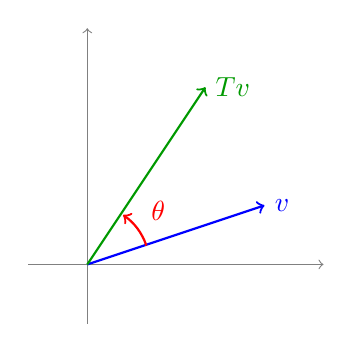
\begin{tikzpicture}[scale=1.5]
    \draw[->, gray] (-0.5, 0) -- (2, 0);
    \draw[->, gray] (0, -0.5) -- (0, 2);
    \draw[->, thick, blue] (0,0) -- (1.5, 0.5) node[right] {$v$};
    \draw[->, thick, green!60!black] (0,0) -- (1.0, 1.5) node[right] {$Tv$};
    \draw[->, red, thick] (0.5, 0.16) arc (18.4:56.3:0.5);
    \node[red] at (0.6, 0.45) {$\theta$};
\end{tikzpicture}
\end{minipage}
\begin{minipage}{0.45\textwidth}
\centering
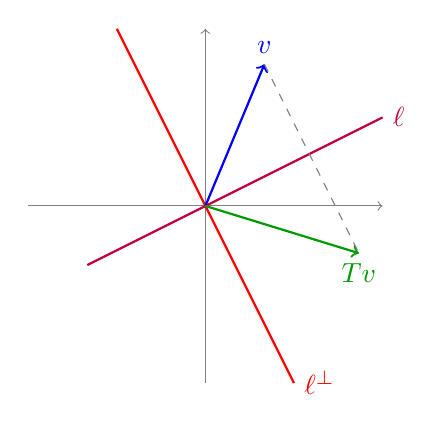
\begin{tikzpicture}[scale=1.5]
    \draw[->, gray] (-1.5, 0) -- (1.5, 0);
    \draw[->, gray] (0, -1.5) -- (0, 1.5);
    \draw[thick, purple] (-1, -0.5) -- (1.5, 0.75) node[right] {$\ell$};
    \draw[thick, red] (-0.75, 1.5) -- (0.75, -1.5) node[right] {$\ell^\perp$};
    \draw[->, thick, blue] (0,0) -- (0.5, 1.2) node[above] {$v$};
    \draw[->, thick, green!60!black] (0,0) -- (1.3, -0.4) node[below] {$Tv$};
    \draw[dashed, gray] (0.5, 1.2) -- (1.3, -0.4);
\end{tikzpicture}
\end{minipage}
\end{center}

\begin{proof}
Note that if $v \in \mathbb{R}^2$ has $\|v\| = 1$, then there exists $\theta \in [0, 2\pi)$ such that $v = \left(\begin{smallmatrix} \cos\theta \\ \sin\theta \end{smallmatrix}\right)$.

Now, let
\[
    A = \begin{pmatrix} | & | \\ u_1 & u_2 \\ | & | \end{pmatrix} \in \Orth(2).
\]
Since $A$ is orthogonal, its columns form an orthonormal basis. Thus, $\|u_1\| = 1$, which implies $u_1 = \left(\begin{smallmatrix} \cos\theta \\ \sin\theta \end{smallmatrix}\right)$ for some $\theta \in [0, 2\pi)$. 
We also have $u_1 \perp u_2$ and $\|u_2\| = 1$. 

The orthogonal complement to $u_1$ is:
\[ \begin{pmatrix} \cos\theta \\ \sin\theta \end{pmatrix}^\perp = \Sp \begin{pmatrix} \cos(\theta + \frac{\pi}{2}) \\ \sin(\theta + \frac{\pi}{2}) \end{pmatrix} = \Sp \begin{pmatrix} -\sin\theta \\ \cos\theta \end{pmatrix}. \]
Within the space $\Sp\left(\begin{smallmatrix} -\sin\theta \\ \cos\theta \end{smallmatrix}\right)$, there are precisely two elements with norm $1$, namely:
\[ u_2' = \begin{pmatrix} -\sin\theta \\ \cos\theta \end{pmatrix}, \quad u_2'' = \begin{pmatrix} \sin\theta \\ -\cos\theta \end{pmatrix}. \]

\begin{center}
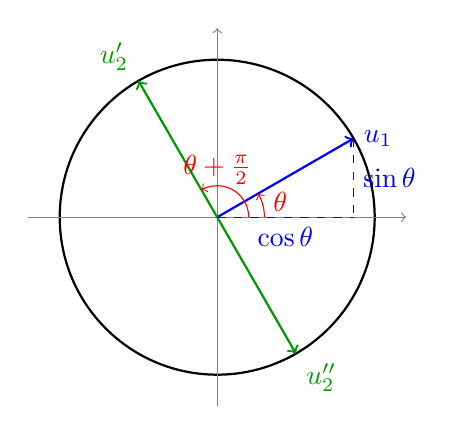
\begin{tikzpicture}[scale=2]
    \draw[thick] (0,0) circle (1cm);
    \draw[->, gray] (-1.2, 0) -- (1.2, 0);
    \draw[->, gray] (0, -1.2) -- (0, 1.2);
    
    \coordinate (U1) at (0.866, 0.5);
    \coordinate (U2P) at (-0.5, 0.866);
    \coordinate (U2PP) at (0.5, -0.866);
    
    \draw[->, thick, blue] (0,0) -- (U1) node[right] {$u_1$};
    \draw[->, thick, green!60!black] (0,0) -- (U2P) node[above left] {$u_2'$};
    \draw[->, thick, green!60!black] (0,0) -- (U2PP) node[below right] {$u_2''$};
    
    \draw[dashed, blue] (U1) -- (0.866, 0) node[midway, right] {$\sin\theta$};
    \draw[dashed, blue] (0,0) -- (0.866, 0) node[midway, below] {$\cos\theta$};
    
    \draw[->, red] (0.3, 0) arc (0:30:0.3);
    \node[red] at (0.4, 0.1) {$\theta$};
    
    \draw[->, red] (0.2, 0) arc (0:120:0.2);
    \node[red] at (0.0, 0.3) {$\theta + \frac{\pi}{2}$};
\end{tikzpicture}
\end{center}

If $u_2 = u_2'$, then $A = \left(\begin{smallmatrix} \cos\theta & -\sin\theta \\ \sin\theta & \cos\theta \end{smallmatrix}\right) = R_\theta$, and $\det A = 1$.

If $u_2 = u_2''$, then $A = \left(\begin{smallmatrix} \cos\theta & \sin\theta \\ \sin\theta & -\cos\theta \end{smallmatrix}\right) = R_\theta \cdot \left(\begin{smallmatrix} 1 & 0 \\ 0 & -1 \end{smallmatrix}\right)$, and $\det A = -1$.

In the second case, a direct calculation shows that $v_1 = \left(\begin{smallmatrix} \cos(\frac{\theta}{2}) \\ \sin(\frac{\theta}{2}) \end{smallmatrix}\right)$ and $v_2 = \left(\begin{smallmatrix} \cos(\frac{\theta}{2} + \frac{\pi}{2}) \\ \sin(\frac{\theta}{2} + \frac{\pi}{2}) \end{smallmatrix}\right)$ are eigenvectors of $A$ for the eigenvalues $\lambda_1 = 1$ and $\lambda_2 = -1$, respectively.
\end{proof}

\begin{summary}
$\SOrth(2) =$ rotations. \\
$\Orth(2) \setminus \SOrth(2) =$ reflections.
\end{summary}

% Cor. (25.a.8)
\begin{corollary}
\label{cor:2d_isometry_matrix}
Let $V$ be a 2-di\-men\-sional Euclidean space and $T \colon V \to V$ a linear isometry. Then $\det(T) = \pm 1$. 
Moreover, there exists an orthonormal basis $\mathcal{B}$ for $V$ such that:
\begin{enumerate}
    \item If $\det(T) = 1$, then $[T]_{\mathcal{B}}^{\mathcal{B}} = R_\theta$.
    \item If $\det(T) = -1$, then $[T]_{\mathcal{B}}^{\mathcal{B}} = \begin{pmatrix} 1 & 0 \\ 0 & -1 \end{pmatrix}$.
\end{enumerate}
\end{corollary}

% Prop. (25.a.9)
\begin{proposition}[Classification of $\SOrth(3)$]
\label{prop:classification_so3}
Let $A \in \SOrth(3)$. Then $1$ is an eigenvalue of $A$. 
Moreover, there exists an orthonormal basis $\mathcal{B} := (v_1, v_2, v_3)$ and $\theta \in [0, 2\pi)$ such that
\[ [T_A]_{\mathcal{B}}^{\mathcal{B}} = \begin{pmatrix} 1 & 0 & 0 \\ 0 & \cos\theta & -\sin\theta \\ 0 & \sin\theta & \cos\theta \end{pmatrix} = \begin{pmatrix} 1 & 0 \\ 0 & R_\theta \end{pmatrix}. \]
So, $T_A$ is a rotation with angle $\theta$ around the axis $\Sp(v_1)$. Moreover:
\begin{enumerate}
    \item If $-1$ is an eigenvalue of $A$, then $\theta = \pi$, hence
    \[ [T_A]_{\mathcal{B}}^{\mathcal{B}} = \begin{pmatrix} 1 & 0 & 0 \\ 0 & -1 & 0 \\ 0 & 0 & -1 \end{pmatrix}. \]
    \item If $-1$ is \emph{not} an eigenvalue of $A$ (which is true if and only if $1$ is the only real eigenvalue), then $\theta \neq \pi$.
\end{enumerate}
\end{proposition}

\begin{center}
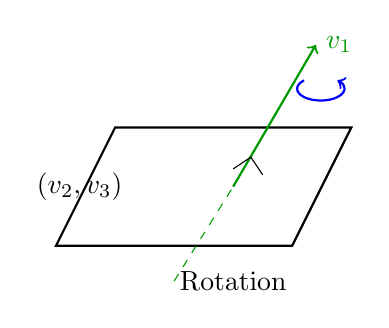
\begin{tikzpicture}[scale=1.5]
    % Plane
    \draw[thick] (-1,-0.5) -- (1,-0.5) -- (1.5, 0.5) -- (-0.5, 0.5) -- cycle;
    \node at (-0.8, 0) {$\Sp(v_2, v_3)$};
    
    % Axis v1
    \draw[->, thick, green!60!black] (0.5, 0) -- (1.2, 1.2) node[right] {$v_1$};
    \draw[dashed, green!60!black] (0, -0.8) -- (0.5, 0);
    
    % Right angle
    \draw (0.5, 0.15) -- (0.65, 0.25) -- (0.75, 0.1);
    
    % Rotation arrow
    \draw[->, thick, blue] (1.1, 0.9) arc (135:405:0.2 and 0.1);
    \node at (0.5, -0.8) {Rotation};
\end{tikzpicture}
\end{center}

\begin{proof}
The characteristic polynomial $P_A(x)$ of $A$ is a polynomial of degree $3$ with real coefficients. By the Intermediate Value Theorem from analysis, any odd-degree polynomial with real coefficients has at least one real zero $\lambda \in \mathbb{R}$ of $P_A(x)$ (i.e., $P_A(\lambda) = 0$). This implies that $A$ has at least one real eigenvalue. 
By a previous theorem (\ref{lem:eigenvalues_orthogonal}), $\lambda = \pm 1$.

Let $v_1 \in \mathbb{R}^3$ be an eigenvector of $\lambda$. By normalizing it if necessary, we may assume $\|v_1\| = 1$. Consider the subspace
\[ L := v_1^\perp = \{v \in \mathbb{R}^3 \mid v \perp v_1\}. \]
Since $A$ is orthogonal, we have for all $v \in L$, $A \cdot v \in L$. (i.e., $T_A(L) \subseteq L$, meaning $L$ is invariant under $T_A$).
Indeed, if $v \in L$, this implies $0 = \langle v, v_1 \rangle$. Because $A \in \Orth(3)$, it preserves inner products:
\[ 0 = \langle v, v_1 \rangle = \langle Av, Av_1 \rangle = \langle Av, \pm v_1 \rangle = \pm \langle Av, v_1 \rangle \implies Av \in L. \]

We also have $\mathbb{R}^3 = \Sp(v_1) \oplus L$, hence $\dim L = 2$.
Now, $T_A|_L \colon L \to L$ is a linear isometry. Let $\mathcal{L} = (w_1, w_2)$ be an orthonormal basis for $L$. By a previous result, the representation matrix is $Q := [T_A|_L]_{\mathcal{L}}^{\mathcal{L}} \in \Orth(2)$.

\textbf{Case (a):} $\lambda = 1$. Take the basis $\mathcal{B} := (v_1, w_1, w_2)$. Then
\[ [T_A]_{\mathcal{B}}^{\mathcal{B}} = \begin{pmatrix} 1 & 0 & 0 \\ 0 & \multicolumn{2}{c}{\multirow{2}{*}{$Q$}} \\ 0 & & \end{pmatrix} = \begin{pmatrix} 1 & 0 \\ 0 & Q \end{pmatrix}. \]
Now, $1 = \det A = \det(T_A) = 1 \cdot \det(Q)$, which implies $\det Q = 1$. 
So, $Q \in \SOrth(2)$. By the previous proposition (\ref{prop:classification_o2}), there exists $\theta \in [0, 2\pi)$ such that $Q = R_\theta$.
Thus,
\[ [T_A]_{\mathcal{B}}^{\mathcal{B}} = \begin{pmatrix} 1 & 0 \\ 0 & R_\theta \end{pmatrix}. \]

\textbf{Case (b):} If $\lambda = -1$. By the same argument as for case (a), we get that $1 = \det A = (-1) \cdot \det(T_A|_L)$, which implies $\det(T_A|_L) = -1$. By \cref{cor:2d_isometry_matrix}, there exists an orthonormal basis $\mathcal{L} = (w_1, w_2)$ for $L$ such that $[T_A|_L]_{\mathcal{L}}^{\mathcal{L}} = \left(\begin{smallmatrix} 1 & 0 \\ 0 & -1 \end{smallmatrix}\right)$.
Take $\mathcal{B}' := (v_1, w_1, w_2)$. Then
\[ [T_A]_{\mathcal{B}'}^{\mathcal{B}'} = \begin{pmatrix} -1 & 0 & 0 \\ 0 & 1 & 0 \\ 0 & 0 & -1 \end{pmatrix}. \]
And for the reordered basis $\mathcal{B} := (w_1, v_1, w_2)$, we have 
\[ [T_A]_{\mathcal{B}}^{\mathcal{B}} = \begin{pmatrix} 1 & 0 & 0 \\ 0 & -1 & 0 \\ 0 & 0 & -1 \end{pmatrix} = \begin{pmatrix} 1 & 0 \\ 0 & R_\pi \end{pmatrix}. \]
Note that in case \textbf{(b)} too, $1$ is an eigenvalue of $A$ (corresponding to the eigenvector $w_1$).
\end{proof}

% Prop. (25.a.10)
\begin{proposition}[Classification of $\Orth(3) \setminus \SOrth(3)$]
\label{prop:classification_o3_minus_so3}
Let $A \in \Orth(3) \setminus \SOrth(3)$. Then there exists an orthonormal basis $\mathcal{B} := (v_1, v_2, v_3)$ for $\mathbb{R}^3$ such that 
\[ [T_A]_{\mathcal{B}}^{\mathcal{B}} = \begin{pmatrix} -1 & 0 & 0 \\ 0 & \cos\theta & -\sin\theta \\ 0 & \sin\theta & \cos\theta \end{pmatrix} = \begin{pmatrix} -1 & 0 \\ 0 & R_\theta \end{pmatrix} \]
for some $\theta \in [0, 2\pi)$. (So $T_A$ does a rotation by $\theta$ around $\Sp(v_1)$, followed by a reflection with respect to $\Sp(v_2, v_3)$).
\end{proposition}

\begin{proof}
Let $A' := -A = (-I) \cdot A$. Then $A' \in \Orth(3)$ and $\det A' = (-1)^3 \cdot \det A = (-1) \cdot (-1) = 1$.
This implies $A' \in \SOrth(3)$. By the previous proposition (\ref{prop:classification_so3}), there exists an orthonormal basis $\mathcal{B}$ for $\mathbb{R}^3$, and $\theta' \in [0, 2\pi)$, such that $[T_{A'}]_{\mathcal{B}}^{\mathcal{B}} = \left(\begin{smallmatrix} 1 & 0 \\ 0 & R_{\theta'} \end{smallmatrix}\right)$. 
This implies:
\begin{align*}
    [T_A]_{\mathcal{B}}^{\mathcal{B}} &= [-\id_{\mathbb{R}^3}]_{\mathcal{B}}^{\mathcal{B}} \cdot [T_{A'}]_{\mathcal{B}}^{\mathcal{B}} \\
    &= -I \cdot \begin{pmatrix} 1 & 0 \\ 0 & R_{\theta'} \end{pmatrix} \\
    &= \begin{pmatrix} -1 & 0 \\ 0 & -R_{\theta'} \end{pmatrix} \\
    &= \begin{pmatrix} -1 & 0 \\ 0 & R_\theta \end{pmatrix},
\end{align*}
where $\theta = (\theta' + \pi) \pmod{2\pi}$. 
(Note that $-R_{\theta'} = R_\pi \circ R_{\theta'} = R_{\theta' + \pi}$).
\end{proof}


\section*{Exercise Solutions}
\addcontentsline{toc}{section}{Exercise Solutions}

\begin{exercisesolution}[Proof of \cref{thm:isometry_equivalences} \textbf{(d)} $\implies$ \textbf{(e)}]
Assume there exists an orthonormal basis $\mathcal{B} = (e_1, \dots, e_n)$ of $V$ such that $Te_1, \dots, Te_n$ is also an orthonormal basis. Since it is an orthonormal basis, we have $\langle Te_i, Te_j \rangle = \delta_{ij}$. 
By the definition of the adjoint map, we can rewrite the inner product as:
\[ \delta_{ij} = \langle Te_i, Te_j \rangle = \langle e_i, T^*Te_j \rangle. \]
Because the vectors $e_i$ form a basis, the fact that the inner product of $T^*Te_j$ with every basis vector $e_i$ yields $\delta_{ij}$ (which are precisely the coordinates of $e_j$) implies that $T^*Te_j = e_j$ for all $1 \leq j \leq n$.
Since the linear map $T^* \circ T$ acts as the identity on a basis, it must be the identity map on the entire space $V$. Thus, $T^* \circ T = \id_V$. (This proves \textbf{(d)} $\implies$ \textbf{(f)}).
Since $V$ is finite-di\-men\-sional, a left inverse is also a right inverse, so $T \circ T^* = \id_V$, proving \textbf{(e)}.
\end{exercisesolution}

\begin{exercisesolution}[Proof of \cref{prop:orth_unitary_matrix_rep}]
Let $\mathcal{B} = (e_1, \dots, e_n)$ be an orthonormal basis for $V$. 
First, suppose $T$ is an orthogonal (resp. unitary) endomorphism. By \cref{thm:isometry_equivalences}, $T \circ T^* = \id_V$ and $T^* \circ T = \id_V$. 
Taking the representation matrix with respect to $\mathcal{B}$, we have:
\[ [T^* \circ T]_{\mathcal{B}}^{\mathcal{B}} = [\id_V]_{\mathcal{B}}^{\mathcal{B}} = I_n. \]
By the properties of representation matrices, this splits into $[T^*]_{\mathcal{B}}^{\mathcal{B}} \cdot [T]_{\mathcal{B}}^{\mathcal{B}} = I_n$. Since $\mathcal{B}$ is an orthonormal basis, $[T^*]_{\mathcal{B}}^{\mathcal{B}} = \left([T]_{\mathcal{B}}^{\mathcal{B}}\right)^*$. 
Thus, $\left([T]_{\mathcal{B}}^{\mathcal{B}}\right)^* \cdot [T]_{\mathcal{B}}^{\mathcal{B}} = I_n$, which means the matrix $[T]_{\mathcal{B}}^{\mathcal{B}}$ is orthogonal (resp. unitary).

Conversely, assume that $A := [T]_{\mathcal{B}}^{\mathcal{B}}$ is orthogonal (resp. unitary). This means $A^* A = I_n$. 
Because $\mathcal{B}$ is an orthonormal basis, $A^* = \left([T]_{\mathcal{B}}^{\mathcal{B}}\right)^* = [T^*]_{\mathcal{B}}^{\mathcal{B}}$. 
Substituting this back yields $[T^*]_{\mathcal{B}}^{\mathcal{B}} \cdot [T]_{\mathcal{B}}^{\mathcal{B}} = I_n$, and therefore $[T^* \circ T]_{\mathcal{B}}^{\mathcal{B}} = [\id_V]_{\mathcal{B}}^{\mathcal{B}}$. This implies the maps are equal, so $T^* \circ T = \id_V$. By \cref{thm:isometry_equivalences}, this guarantees $T$ is an isometry.
\end{exercisesolution}

\begin{exercisesolution}[Proof of \cref{prop:group_properties}]
We will prove this generically for $G = \Unit(n)$ and $G = \SUnit(n)$ (the real cases are identical, replacing the conjugate transpose $^*$ with the transpose $\transp$).
\begin{enumerate}[label=\textbf{(\alph*)}]
    \item The identity matrix $I_n$ satisfies $I_n^* \cdot I_n = I_n \cdot I_n = I_n$, so $I_n \in \Unit(n)$. Furthermore, $\det(I_n) = 1$, so $I_n \in \SUnit(n)$.
    
    \item Let $A, B \in \Unit(n)$. We evaluate $(AB)^* (AB) = (B^* A^*) (AB) = B^* (A^* A) B$. Since $A \in \Unit(n)$, $A^* A = I_n$, so this reduces to $B^* I_n B = B^* B$. Since $B \in \Unit(n)$, $B^* B = I_n$. Thus, $AB \in \Unit(n)$. 
    If additionally $A, B \in \SUnit(n)$, then $\det(AB) = \det(A)\det(B) = 1 \cdot 1 = 1$, so $AB \in \SUnit(n)$.
    
    \item Let $A \in \Unit(n)$. This implies $A^* A = I_n$, meaning $A^{-1} = A^*$. We check if $A^{-1}$ is unitary: $(A^{-1})^* A^{-1} = (A^*)^* A^* = A A^* = I_n$. Thus, $A^{-1} \in \Unit(n)$. 
    If additionally $A \in \SUnit(n)$, then $\det(A^{-1}) = \frac{1}{\det(A)} = \frac{1}{1} = 1$, so $A^{-1} \in \SUnit(n)$.
\end{enumerate}
\end{exercisesolution}